\documentclass{article}
\usepackage{tikz}
\usetikzlibrary{decorations.pathreplacing}
\usepackage{amsmath}
\usepackage[a4paper]{geometry}
\usepackage{fancyhdr}
\pagestyle{fancy}
\lhead{Magnetische Flussdichten}
\rhead{September 2025}
\newcommand{\ounit}[1]{
 1\,\text{#1} 
} 
 
\begin{document}
\section{Magnetische Flussdichten}
\begin{minipage}{\dimexpr\linewidth-5cm} 
Die \emph{magnetische Flussdichte} $B$ beschreibt die Stärke eines Magnetfeldes. Für ein magnetisches Feld, in welchem ein elektrischer Leiter ist, gilt
\[
 B = \frac{F_L}{I \cdot l} 
 \quad \text{mit $l$ als Länge des Leiters} 
\]
Somit ist die magnetische Flussdichte $B$ sehr ähnlich zur elektrischen Feldstärke $E$, so dass beides die wirkende Kraft pro einer elektrischen Größe darstellt. \newline
\end{minipage} 
\hfill
\begin{minipage}{5cm}
 \center
 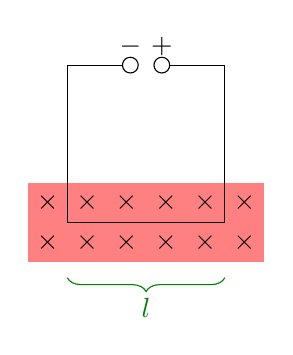
\begin{tikzpicture}
  \fill[red!50] (-1.5, -1.5) rectangle (1.5, -2.5);
  \foreach \x in {-3,...,2} {
   \foreach \y in {0,1} {
    \draw (\x*0.5+0.25, \y*0.5-2.25) node{$\times$};
   };
  };
 
  \draw (-0.2, 0) circle (0.1cm) node[above] {$-$};
  \draw (0.2, 0) circle (0.1cm) node[above] {$+$};
  \draw (-0.3, 0) -- (-1, 0);
  \draw (0.3, 0) -- (1, 0);
  \draw (-1, 0) -- (-1, -2);
  \draw (1, 0) -- (1, -2);
  \draw (-1, -2) -- (1, -2); 
 
  \draw [green!50!black, decorate,decoration={brace,amplitude=5pt,mirror}]
  (-1,-2.7) -- (1,-2.7) node[midway,below,yshift=-4pt]{$l$};
 \end{tikzpicture} 
\end{minipage}
$B$ wird dabei in der Einheit Tesla $T$ angegeben, wobei, aus der obigen Formel offensichtlich,
\[ 
 \ounit{Tesla} = \frac{\ounit{Newton}}{\ounit{Ampere} \cdot \ounit{Meter}}
\]
 
\subsection{Stromwaage}
Eine Stromwaage ist ein Messgerät, welches die Lorentzkraft misst und somit genutzt werden, um, mit der obigen Formel, die magnetische Flussdichte zu bestimmen. % TODO: erläutern können \newline
Messungen einer Stromwaage zeigen, dass die Kraft proportional zur Länge $l$, der magnetischen Flussdichte und der Stromstärke ist.   
\end{document}